
\documentclass[12pt, a4paper]{article}
\usepackage{fullpage}
\usepackage{graphicx}
\usepackage{wrapfig}
\usepackage{amsmath}
\usepackage{float}
\usepackage{listings}
\usepackage{lmodern}  % for bold teletype font
\usepackage{xcolor}   % for \textcolor

\definecolor{codegreen}{rgb}{0,0.6,0}
\definecolor{codegray}{rgb}{0.5,0.5,0.5}
\definecolor{codepurple}{rgb}{0.58,0,0.82}
\definecolor{backcolour}{rgb}{0.95,0.95,0.92}

\title{\textbf{EE2703 : Applied Programming Lab \\ Assignment 6}} % Title

\author{Potta Muni Asheesh \\ EE19B048} % Author name

\date{\today} % Date for the report

\begin{document}	
\lstset{
  language=Python,
  backgroundcolor=\color{backcolour},   
  commentstyle=\color{codegreen},
  keywordstyle=\color{magenta},
  numberstyle=\tiny\color{codegray},
  stringstyle=\color{codepurple},
  basicstyle=\ttfamily,
  breakatwhitespace=false,         
  breaklines=true,                 
  captionpos=b,                    
  keepspaces=true,                 
  %numbers=left,                    
  %numbersep=5pt,                  
  showspaces=false,                
  showstringspaces=false,
  showtabs=false,                  
  tabsize=2,
  columns=fullflexible,
  frame=single,
  postbreak=\mbox{\textcolor{red}{$\hookrightarrow$}\space},
}	
		
\maketitle % Insert the title, author and date

\section{Introduction}

In this assignment, the \texttt{signal} toolbox available in scipy is explored.

\section{Q1}

It is asked to solve for the time response of a spring whose motion is described by the following differential equation.
\begin{equation*}
\ddot{x} + 2.25x = f(t)
\end{equation*}
It is given that $f(t) = e^{-0.5t}cos(1.5t)u(t)$, whose Laplace transform is given by
\begin{equation*}
F(s) = \frac{s+0.5}{(s+0.5)^2 + 2.25}
\end{equation*}
Applying laplace transform on the differential equation with the given initial conditions, we get the laplace transform of $x$ as
\begin{align*}
s^2 X(s) + 2.25X(s) &= F(s) \\
\implies X(s) &= \frac{F(s)}{s^2 + 2.25} \\
\implies X(s) &= \frac{s + 0.5}{(s^2 + 2.25)((s+0.5)^2 + 2.25)}
\end{align*}
A system is to be defined whose transfer function is $X(s)$ so that $x(t)$ can be obtained finding the impulse response of the system. To do the polynomial multiplication in the denominator \texttt{polymul} is used and \texttt{impulse} is used to find the impulse response.
\begin{lstlisting}
def q1_q2(a=0.5):
    Num = np.array([1, a])
    Den = np.polymul([1, 2*a, 2.25+(a*a)], [1, 0, 2.25])
    H = sp.lti(Num, Den)
    t, x = sp.impulse(H, None, np.linspace(0, 50, 501))\\
    global fignum
    plt.figure(fignum)
    fignum += 1
    plt.plot(t, x)
    plt.title(r'Undamped forced oscillation with $f(t) = cos(1.5t) e^{-at} u_0(t)$')
\end{lstlisting}
The plot of the $x(t)$ is given below.
\begin{figure}[H]
\centering
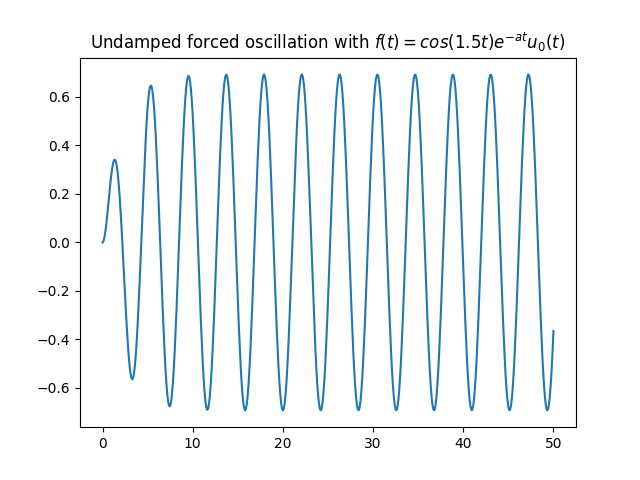
\includegraphics[width=0.8\textwidth]{Figure_1.png}
\caption{Forced undamped oscillations}
\end{figure}

\section{Q2}

If $f(t) = e^{-0.05t}cos(1.5t)u(t)$, then the force acting on the spring decays slowly, so the system has more time to resonate with the force and the amplitude of the oscillations increases significantly. The plot is given below.
\begin{figure}[H]
\centering
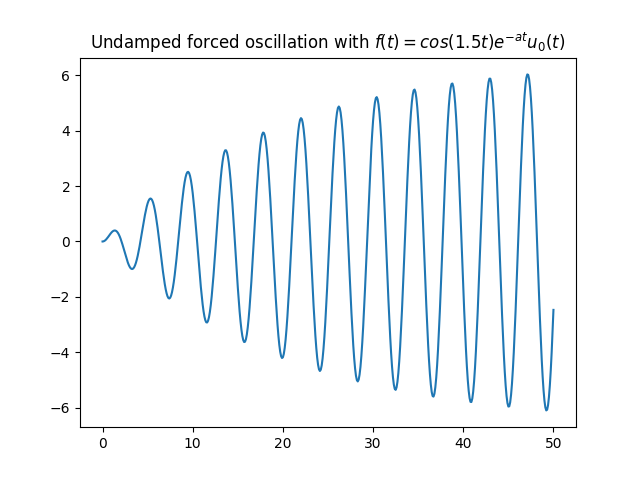
\includegraphics[width=0.8\textwidth]{Figure_2.png}
\caption{Forced undamped oscillations}
\end{figure}


\section{Q3}

If $f(t)$ is treated as input and $x(t)$ as output, then the system transfer function becomes
\begin{equation*}
\frac{X(s)}{F(s)} = \frac{1}{s^2 + 2.25}
\end{equation*}
The output for a certain input can be obtained by using \texttt{lsim}. The input is taken as $f(t) = e^{-0.05t}cos(\omega t)u(t)$ and the frequency of the cosine term ($\omega$) is varied from 1.4 to 1.6 in steps of 0.05 and the corresponding plots are given below.
\begin{lstlisting}
def q3():
    H = sp.lti([1], [1, 0, 2.25])
    global fignum
    t = np.linspace(0, 50, 501)
    for w in np.arange(1.4, 1.6, 0.05):
        f = np.cos(w*t)*np.exp(-0.05*t)
        t, x = sp.lsim(H, f, t)[:2]
        plt.figure(fignum)
        fignum += 1
        plt.plot(t, x, label=r'$\omega$'+' = %.2f'%(w))
        plt.title(r'Variation with frequency')
        plt.legend()
\end{lstlisting}
\begin{figure}[H]
\centering
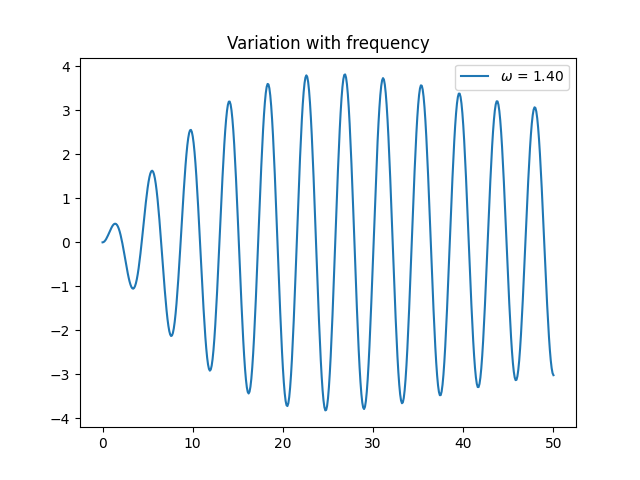
\includegraphics[width=0.8\textwidth]{Figure_3.png}
\caption{Forced undamped oscillations $\omega = 1.4$}
\end{figure}
\begin{figure}[H]
\centering
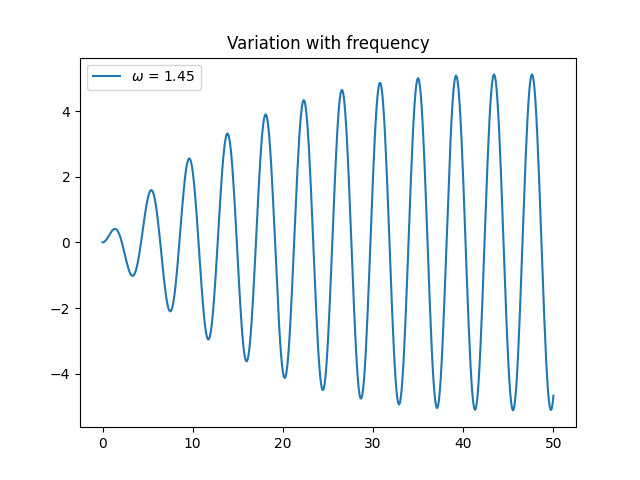
\includegraphics[width=0.8\textwidth]{Figure_4.png}
\caption{Forced undamped oscillations $\omega = 1.45$}
\end{figure}
\begin{figure}[H]
\centering
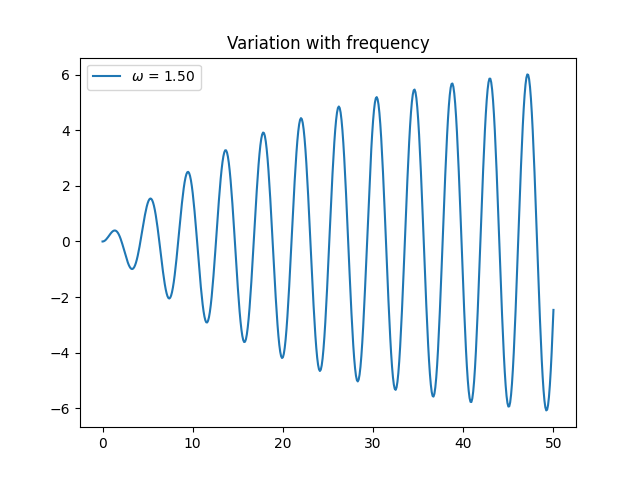
\includegraphics[width=0.8\textwidth]{Figure_5.png}
\caption{Forced undamped oscillations $\omega = 1.5$}
\end{figure}
\begin{figure}[H]
\centering
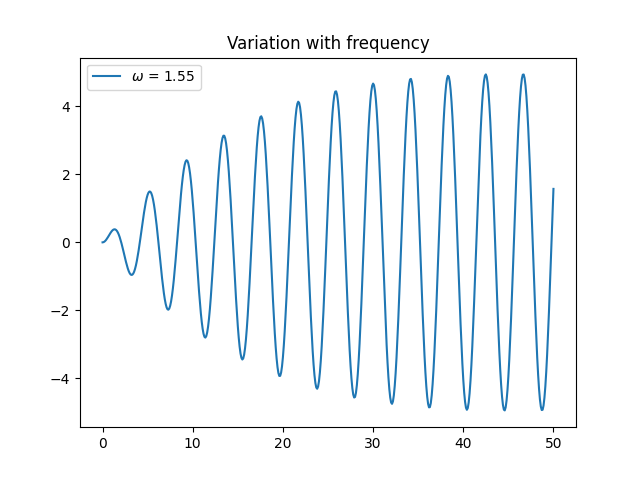
\includegraphics[width=0.8\textwidth]{Figure_6.png}
\caption{Forced undamped oscillations $\omega = 1.55$}
\end{figure}
\begin{figure}[H]
\centering
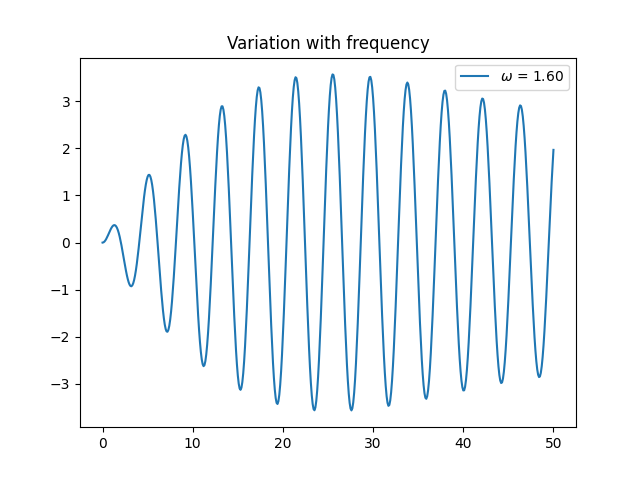
\includegraphics[width=0.8\textwidth]{Figure_7.png}
\caption{Forced undamped oscillations $\omega = 1.6$}
\end{figure}
It is observed that the amplitude of oscillations increases from $\omega = 1.4$ to $\omega = 1.5$ and then decreases. So, the peak amplitude is seen at 1.5 rad/s. This happens as the natural frequency of the system is 1.5rad/s and when the input is also at the same frequency, the system resonates.

\section{Q4 - Coupled spring problem}

From the given coupled spring problem, when the equations are decoupled, the resulting equations are
\begin{align*}
\ddddot{x} + 3\ddot{x} &= 0 \\
\ddot{x} + x &= y
\end{align*}
and the initial conditions are, $x(0) = 1, \dot{x}(0) = 0, \ddot{x}(0) = -1, \dddot{x}(0) = 0$. Upon finding the laplace transform along with initial conditions, they are given by
\begin{align*}
X(s) &= \frac{s^2 + 2}{s^3 + 3s} \\
Y(s) &= \frac{2}{s^3 + 3s}\\
X(s) &= \frac{2}{3s}+\frac{1}{3(s^2 +3)} \\
Y(s) &= \frac{2}{3s} - \frac{2s}{3(s^2+3)}
\end{align*}
Applying inverse laplace transform on $X(s)$ and $Y(s)$, $x(t)$ and $y(s)$ are given by
\begin{align*}
x(t) &= (\frac{2}{3} + \frac{1}{3}cos(\sqrt{3}t))u(t) \\
y(t) &= \frac{2}{3}(1-cos(\sqrt{3}t))u(t)
\end{align*}
A system can generated for both $X(s)$ and $Y(s)$ and \texttt{impulse} can be used to get $x(t)$ and $y(t)$. The plot is given below.
\begin{lstlisting}
def q4():
    X = sp.lti([1, 0, 2], [1, 0, 3, 0])
    Y = sp.lti([2], [1, 0, 3, 0])
    t = np.linspace(0, 20, 201)
    t, x = sp.impulse(X, None, t)
    t, y = sp.impulse(Y, None, t)
    global fignum
    plt.figure(fignum)
    fignum += 1
    plt.plot(t, x, 'r', label='x(t)')
    plt.plot(t, y, 'g', label='y(t)')
    plt.title('Q4: Solutions of the coupled spring problem')
    plt.legend()
\end{lstlisting}
\begin{figure}[H]
\centering
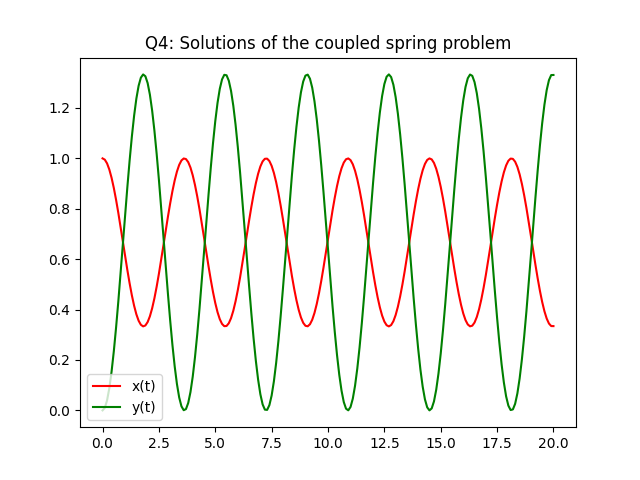
\includegraphics[width=0.8\textwidth]{Figure_8.png}
\caption{Coupled spring oscillations}
\end{figure}

\section{Q5 - Series RLC Circuit}

A series RLC circuit is given and output is voltage across the capacitor C. The steady state transfer function is given by,
\begin{equation*}
H(s) = \frac{1}{1 + sRC + s^2LC}
\end{equation*}
where, $R = 100\Omega$, $L = 1\mu H$, $C = 1\mu F$, so the transfer function can be approximated as,
\begin{equation*}
H(s) = \frac{1}{(1+10^{-4}s)(1+10^{-8}s)}
\end{equation*}
The poles are at $s = -10^4, -10^8$
The plot of magnitude and phase response is given below.
\begin{figure}[H]
\centering
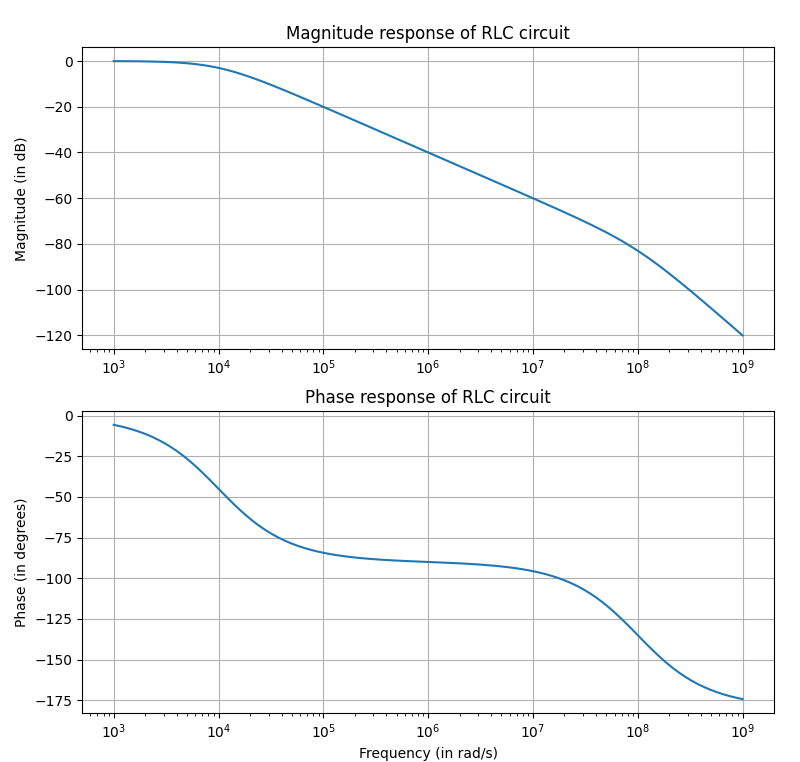
\includegraphics[width=0.8\textwidth]{Figure_9.png}
\caption{Frequency response of RLC circuit}
\end{figure}

\section{Q6 - Filtering using RLC circuit}

When input $v_i(t) = (cos(10^3t) - cos(10^6t))u(t)$, the system response is found using \texttt{lsim}. The output response $v_o(t)$ consists  of two parts, the transient response and the steady state response. The transient response is observed for $t < 30\mu s$ and it decays as the time increases. The steady state response can be observed for $t < 10ms$. The plots for both are given below.
\begin{figure}[H]
\centering
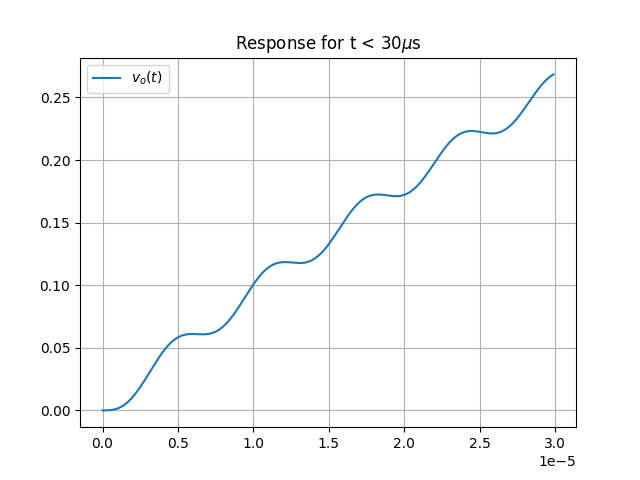
\includegraphics[width=0.8\textwidth]{Figure_10.png}
\caption{Transient response}
\end{figure}\begin{figure}[H]
\centering
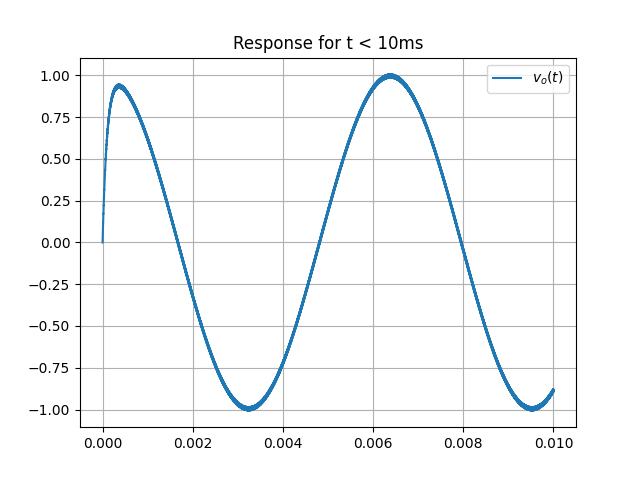
\includegraphics[width=0.8\textwidth]{Figure_11.png}
\caption{Steady state response}
\end{figure}
The transient response involves the transition from initial conditions to steady state. The initial conditions are taken as $v_o(0) = 0, \dot{v_o}(0) = 0$. In the steady state, the high frequency component($\omega	= 10^6 rad/s$) of input is suppressed and the lower frequency component is allowed to output. This is evident from the frequency response. This is the filtering action of series RLC circiut.

\begin{lstlisting}
def q5_q6():
    H = sp.lti([1], [1e-12, 1e-4, 1])
    w, mag, phi = H.bode()
    global fignum
    plt.figure(fignum,figsize=(8,6))
    fignum += 1
    plt.subplot(2, 1, 1)
    # plt.tight_layout()
    plt.title('Magnitude response of RLC circuit')
    plt.semilogx(w, mag)
    plt.grid(True)
    plt.ylabel('Magnitude (in dB)')
    plt.subplot(2, 1, 2)
    plt.tight_layout()
    plt.title('Phase response of RLC circuit')
    plt.semilogx(w, phi)
    plt.grid(True)
    plt.ylabel('Phase (in degrees)')
    plt.xlabel('Frequency (in rad/s)')

    t = np.arange(0, 1e-2, 1e-7)
    vi = np.cos(1e3*t) - np.cos(1e6*t)
    t, vo = sp.lsim(H, vi, t)[:2]
    plt.figure(fignum)
    fignum += 1
    plt.plot(t[:300], vo[:300], label=r'$v_o(t)$')
    plt.grid(True)
    plt.legend()
    plt.title(r'Response for t < 30$\mu$s')
    plt.figure(fignum)
    fignum += 1
    plt.plot(t, vo, label=r'$v_o(t)$')
    plt.grid(True)
    plt.legend()
    plt.title(r'Response for t < 10ms')
\end{lstlisting}

\end{document} 
